\sectionthree{Myhill--Nerode theorem for regularity and DFA minimization}
\begin{python0}
  from solutions import *; clear()
\end{python0}
% http://theory.stanford.edu/~trevisan/cs154-12/notemindfa.pdf
% https://cs.stackexchange.com/questions/44012/algorithms-for-minimizing-moore-automata


PUT SOMEWHERE: Go ahead and review equivalence relations.

Here's the aim: Let $M$ be a DFA. Can we find another DFA $M'$ such
that
\begin{itemize}
\item $L(M') = L(M)$
\item $M'$ is a DFA with the smallest number of states satisfying
  the above.
\end{itemize}
In other words I want to minimize $M$.

Why would you want to do that?
Because a smaller DFA will execute faster and
furthermore will require less memory (states are memory)
and therefore cheaper to produce.
This is the case whether the DFA is a piece of software
or a piece of hardware.
Therefore DFA minimization improves runtime, space,
and cost.

I will say that two automatas are \defone{equivalent} (whether they
are DFAs or NFAs) if they
accept the same language.

\begin{ex}
  Create three equivalent DFAs
  where
  one has two states, one has 3 states, and the last has 5 states.
  Prove that the one with two states is the minimal, i.e.,
  you cannot find another DFA that accepts the same language
  and has 1 state.
  You have 2 minutes.
  \qed
\end{ex}

The main result is this:

\begin{thm}
  For any DFA, there is a minimum equivalent DFA that is unique
  up to relabeling of states.
\end{thm}

The result is not just \lq\lq there is a minimal DFA".
There are algorithms for converting a given DFA to a smallest one.
I don't have time to talk about all of them.
I'll focus on just one.
And before explaining the algorithm, I'll do one example
first so you get the main idea.
Before that, I'll talk about isomorphism of DFAs.

In computer science and math, two objects of the same kind
is said to be isomorphic (example: graph isomorphism)
if they are essentially the same except for some renaming
of the internals of the objects.
You can also define isomorphism of DFAs.
In that case, you can restate the theorem as saying that the
minimal DFA exist and is unique up to isomorphism.
Here's the formal definition of DFA isomorphism:
Two DFAs
$M = (\Sigma, Q, q_0, F, \delta)$
and
$M' = (\Sigma, Q', q'_0, F', \delta')$
are \defterm{isomorphic} if there is a bijection
\[
f: Q \rightarrow Q'
\]
($f$ is the renaming)
such that
\begin{align*}
f(q_0) = q'_0 \\
f(F) = F' 
\end{align*}
and
\[
\delta(q_i, x) = q_j
\iff
\delta(f(q_i), x) = f(q_j)
\]
You can see that $f$ is just a re-labeling of states
so that the \lq\lq behavior" of the states remain the same.
For instance
\[
f(q_0) = q'_0
\]
means that the start state of $M$ has been renamed as the start state
of $M'$.
The condition
\[
f(F) = F'
\]
means that if a state $q$ in $M$ is an accept state,
then after being renamed to $f(q)$ in $M'$, $f(q)$ is also an accept
state in $M'$.
The transition function renaming is a little bit more complicated.
The condition
\[
\delta(q_i, x) = q_j
\iff
\delta(f(q_i), x) = f(q_j)
\]
means that if at state $q_i$, on reading a character $x$,
you transition to $q_j$, then after renaming
$q_i$ to $f(q_i)$
and
$q_j$ to $f(q_j)$,
at state $f(q_i)$, on reading $x$, you also transition to
state $f(q_j)$ (and vice versa).

Note that the alphabet is the same for $M$ and $M'$.
You can also talk about relabeling (or renaming) of alphabet too.

The general idea of isomorphism is extremely important in
computer science and math (and therefore is also use heavily in
physics, chemistry, engineering, etc.)

Note that the above talks about \lq\lq sameness" in two different
ways: equivalence of DFAs and isomorphism of DFAs.
Isomorphism of DFAs is stronger.


\newpage

\begin{ex}
  Consider the following two DFAs:
\begin{center}
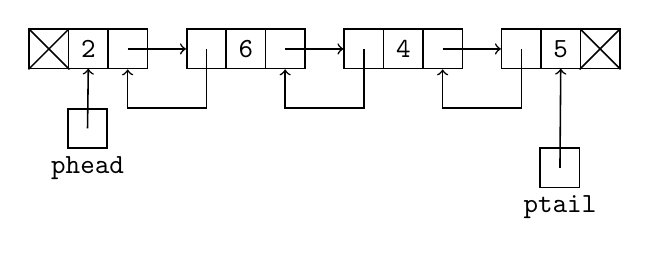
\begin{tikzpicture}

\draw (0.25, 0.25)
  node[draw, line width=0.02cm, , color=black,
       rounded corners=0cm, inner sep=0cm] {

\begin{minipage}[t][0.5cm]{0.5cm}
\mbox{}

\end{minipage}

};\draw (0.25, 0.25) node[color=black] {{\texttt{}}};
\draw (0.75, 0.25)
  node[draw, line width=0.02cm, , color=black,
       rounded corners=0cm, inner sep=0cm] {

\begin{minipage}[t][0.5cm]{0.5cm}
\mbox{}

\end{minipage}

};\draw (0.75, 0.25) node[color=black] {{\texttt{2}}};
\draw (1.25, 0.25)
  node[draw, line width=0.02cm, , color=black,
       rounded corners=0cm, inner sep=0cm] {

\begin{minipage}[t][0.5cm]{0.5cm}
\mbox{}

\end{minipage}

};\draw (1.25, 0.25) node[color=black] {{\texttt{}}};
\draw (2.25, 0.25)
  node[draw, line width=0.02cm, , color=black,
       rounded corners=0cm, inner sep=0cm] {

\begin{minipage}[t][0.5cm]{0.5cm}
\mbox{}

\end{minipage}

};\draw (2.25, 0.25) node[color=black] {{\texttt{}}};
\draw (2.75, 0.25)
  node[draw, line width=0.02cm, , color=black,
       rounded corners=0cm, inner sep=0cm] {

\begin{minipage}[t][0.5cm]{0.5cm}
\mbox{}

\end{minipage}

};\draw (2.75, 0.25) node[color=black] {{\texttt{6}}};
\draw (3.25, 0.25)
  node[draw, line width=0.02cm, , color=black,
       rounded corners=0cm, inner sep=0cm] {

\begin{minipage}[t][0.5cm]{0.5cm}
\mbox{}

\end{minipage}

};\draw (3.25, 0.25) node[color=black] {{\texttt{}}};
\draw (4.25, 0.25)
  node[draw, line width=0.02cm, , color=black,
       rounded corners=0cm, inner sep=0cm] {

\begin{minipage}[t][0.5cm]{0.5cm}
\mbox{}

\end{minipage}

};\draw (4.25, 0.25) node[color=black] {{\texttt{}}};
\draw (4.75, 0.25)
  node[draw, line width=0.02cm, , color=black,
       rounded corners=0cm, inner sep=0cm] {

\begin{minipage}[t][0.5cm]{0.5cm}
\mbox{}

\end{minipage}

};\draw (4.75, 0.25) node[color=black] {{\texttt{4}}};
\draw (5.25, 0.25)
  node[draw, line width=0.02cm, , color=black,
       rounded corners=0cm, inner sep=0cm] {

\begin{minipage}[t][0.5cm]{0.5cm}
\mbox{}

\end{minipage}

};\draw (5.25, 0.25) node[color=black] {{\texttt{}}};
\draw (6.25, 0.25)
  node[draw, line width=0.02cm, , color=black,
       rounded corners=0cm, inner sep=0cm] {

\begin{minipage}[t][0.5cm]{0.5cm}
\mbox{}

\end{minipage}

};\draw (6.25, 0.25) node[color=black] {{\texttt{}}};
\draw (6.75, 0.25)
  node[draw, line width=0.02cm, , color=black,
       rounded corners=0cm, inner sep=0cm] {

\begin{minipage}[t][0.5cm]{0.5cm}
\mbox{}

\end{minipage}

};\draw (6.75, 0.25) node[color=black] {{\texttt{5}}};
\draw (7.25, 0.25)
  node[draw, line width=0.02cm, , color=black,
       rounded corners=0cm, inner sep=0cm] {

\begin{minipage}[t][0.5cm]{0.5cm}
\mbox{}

\end{minipage}

};\draw (7.25, 0.25) node[color=black] {{\texttt{}}};\draw[line width=0.02cm,black,->] (1.25,0.25) to  (1.99,0.25);
\draw[line width=0.02cm,black,->] (3.25,0.25) to  (3.99,0.25);
\draw[line width=0.02cm,black,->] (2.25,0.25) to  (2.25,-0.5) to  (1.25,-0.5) to  (1.25,-0.01);
\draw[line width=0.02cm,black,->] (5.25,0.25) to  (5.99,0.25);
\draw[line width=0.02cm,black,->] (4.25,0.25) to  (4.25,-0.5) to  (3.25,-0.5) to  (3.25,-0.01);
\draw[line width=0.02cm,black,->] (6.25,0.25) to  (6.25,-0.5) to  (5.25,-0.5) to  (5.25,-0.01);
\draw[line width=0.02cm,black] (-0.01,0.51) to  (0.51,-0.01);
\draw[line width=0.02cm,black] (0.51,0.51) to  (-0.01,-0.01);
\draw[line width=0.02cm,black] (6.99,0.51) to  (7.51,-0.01);
\draw[line width=0.02cm,black] (7.51,0.51) to  (6.99,-0.01);

\draw (0.74, -0.76)
  node[draw, line width=0.02cm, , color=black,
       rounded corners=0cm, inner sep=0cm] {

\begin{minipage}[t][0.5cm]{0.5cm}
\mbox{}

\end{minipage}

};\draw (0.74, -0.76) node[color=black] {{\texttt{}}};
\draw (0.74, -1.26)
  node[draw, line width=0.02cm, , color=white,
       rounded corners=0cm, inner sep=0cm] {

\begin{minipage}[t][0.1cm]{0.1cm}
\mbox{}

\end{minipage}

};\draw (0.74, -1.26) node[color=black] {{\texttt{phead}}};\draw[line width=0.02cm,black,->] (0.74,-0.76) to  (0.75,0);

\draw (6.74, -1.26)
  node[draw, line width=0.02cm, , color=black,
       rounded corners=0cm, inner sep=0cm] {

\begin{minipage}[t][0.5cm]{0.5cm}
\mbox{}

\end{minipage}

};\draw (6.74, -1.26) node[color=black] {{\texttt{}}};
\draw (6.74, -1.76)
  node[draw, line width=0.02cm, , color=white,
       rounded corners=0cm, inner sep=0cm] {

\begin{minipage}[t][0.1cm]{0.1cm}
\mbox{}

\end{minipage}

};\draw (6.74, -1.76) node[color=black] {{\texttt{ptail}}};\draw[line width=0.02cm,black,->] (6.74,-1.26) to  (6.75,0);
\end{tikzpicture}

\end{center}


from latextool_basic import *
print(automata(layout="""
A  B   C  D
""",
edges="A,$a$,B|A,$b$,D|B,$a$,B|B,$b$,C|C,$a$,A|C,$b$,B|D,$a$,B|D,$b$,C",
A='initial|label=$0$',
B='label=$1$',
C='label=$2$',
D='accept|label=$3$',
))
\end{python}
and
\begin{comment}
\begin{center}
\begin{tikzpicture}

\fill[white] (19.0, -0.6) circle (0.3);
\node [line width=0.03cm,black,minimum size=0.57cm,draw,circle] at (19.0,-0.6)(A){};\draw (19.0, -0.6) node[color=black] {\texttt{20}};
\fill[white] (16.0, -1.0) circle (0.3);
\node [line width=0.03cm,black,minimum size=0.57cm,draw,circle] at (16.0,-1.0)(a){};\draw (16.0, -1.0) node[color=black] {\texttt{10}};
\fill[white] (10.0, -2.0) circle (0.3);
\node [line width=0.03cm,black,minimum size=0.57cm,draw,circle] at (10.0,-2.0)(b){};\draw (10.0, -2.0) node[color=black] {\texttt{0}};
\fill[white] (11.0, -4.0) circle (0.3);
\node [line width=0.03cm,black,minimum size=0.57cm,draw,circle] at (11.0,-4.0)(d){};\draw (11.0, -4.0) node[color=black] {\texttt{18}};
\fill[white] (8.0, -3.0) circle (0.3);
\node [line width=0.03cm,black,minimum size=0.57cm,draw,circle] at (8.0,-3.0)(e){};\draw (8.0, -3.0) node[color=black] {\texttt{-2}};
\fill[white] (7.0, -4.0) circle (0.3);
\node [line width=0.03cm,black,minimum size=0.57cm,draw,circle] at (7.0,-4.0)(k){};\draw (7.0, -4.0) node[color=black] {\texttt{-3}};
\fill[white] (9.0, -4.0) circle (0.3);
\node [line width=0.03cm,black,minimum size=0.57cm,draw,circle] at (9.0,-4.0)(l){};\draw (9.0, -4.0) node[color=black] {\texttt{-1}};
\fill[white] (15.0, -4.0) circle (0.3);
\node [line width=0.03cm,black,minimum size=0.57cm,draw,circle] at (15.0,-4.0)(h){};\draw (15.0, -4.0) node[color=black] {\texttt{8}};
\fill[white] (14.0, -5.0) circle (0.3);
\node [line width=0.03cm,black,minimum size=0.57cm,draw,circle] at (14.0,-5.0)(m){};\draw (14.0, -5.0) node[color=black] {\texttt{6}};
\fill[white] (13.0, -3.0) circle (0.3);
\node [line width=0.03cm,black,minimum size=0.57cm,draw,circle] at (13.0,-3.0)(f){};\draw (13.0, -3.0) node[color=black] {\texttt{5}};
\fill[white] (13.0, -6.0) circle (0.3);
\node [line width=0.03cm,black,minimum size=0.57cm,draw,circle] at (13.0,-6.0)(n){};\draw (13.0, -6.0) node[color=black] {\texttt{4}};
\fill[white] (15.0, -6.0) circle (0.3);
\node [line width=0.03cm,black,minimum size=0.57cm,draw,circle] at (15.0,-6.0)(o){};\draw (15.0, -6.0) node[color=black] {\texttt{7}};
\fill[white] (18.0, -2.0) circle (0.3);
\node [line width=0.03cm,black,minimum size=0.57cm,draw,circle] at (18.0,-2.0)(p){};\draw (18.0, -2.0) node[color=black] {\texttt{15}};\draw[line width=0.03cm,black,->,>=triangle 60] (A) to  (a);
\draw[line width=0.03cm,black,->,>=triangle 60] (a) to  (p);
\draw[line width=0.03cm,black,->,>=triangle 60] (a) to  (b);
\draw[line width=0.03cm,black,->,>=triangle 60] (b) to  (e);
\draw[line width=0.03cm,black,->,>=triangle 60] (b) to  (f);
\draw[line width=0.03cm,black,->,>=triangle 60] (f) to  (d);
\draw[line width=0.03cm,black,->,>=triangle 60] (f) to  (h);
\draw[line width=0.03cm,black,->,>=triangle 60] (e) to  (k);
\draw[line width=0.03cm,black,->,>=triangle 60] (e) to  (l);
\draw[line width=0.03cm,black,->,>=triangle 60] (h) to  (m);
\draw[line width=0.03cm,black,->,>=triangle 60] (m) to  (n);
\draw[line width=0.03cm,black,->,>=triangle 60] (m) to  (o);
\end{tikzpicture}

\end{center}


from latextool_basic import *
print(automata(layout="""
   D
A     B
   C   
""",
edges="A,$a$,B|A,$b$,D|B,$a$,B|B,$b$,C|C,$a$,A|C,$b$,B|D,$a$,B|D,$b$,C",
A='initial|label=$A$',
B='label=$C$',
C='label=$D$',
D='accept|label=$B$',
))
\end{python}
\end{comment}
\begin{center}
\begin{tikzpicture}[>=triangle 60,shorten >=0.5pt,node distance=2cm,auto,initial text=]
\node[state,accepting] (D) at (  3,  0) {$B$};
\node[state,initial] (A) at (  0, -2) {$A$};
\node[state] (B) at (  6, -2) {$C$};
\node[state] (C) at (  3, -4) {$D$};

\path[->]
(A) edge [bend left=0,pos=0.25,above] node {$a$} (B)
(A) edge [bend left=0,pos=0.5,above] node {$b$} (D)
(B) edge [loop above] node {$a$} ()
(B) edge [bend left=10,pos=0.5] node {$b$} (C)
(C) edge [bend left=0,pos=0.5] node {$a$} (A)
(C) edge [bend left=10,pos=0.5,above] node {$b$} (B)
(D) edge [bend left=0,pos=0.5,above] node {$a$} (B)
(D) edge [bend left=0,pos=0.25] node[pos=0.25] {$b$} (C)
;
\end{tikzpicture}
\end{center}
Are they isomorphic?
\qed
\end{ex}

\newpage
\begin{ex}
  \mbox{}
  \begin{tightlist}
  \item True or false:
    \begin{tightlist}
    \item If $M, M'$ are equivalent DFAs, then they are isomorphic.
    \item If $M, M'$ are isomorphic DFAs, then they are equivalent.
    \end{tightlist}
  \item Is equivalence of DFAs an equivalent relation?
  \item Is isomorphism of DFAs an equivalent relation?  
  \end{tightlist}
  \qed
\end{ex}


\newpage
\begin{ex}
  What is the right definition of isomorphism
  if you want to rename the symbols in alphabets as well?
  (There's only one reasonable definition.)
  The definition should look like this:
  \lq\lq An isomorphism between two DFAs
  $M = (\Sigma, Q, q_0, F, \delta)$
  and
  $M' = (\Sigma', Q', q'_0, F', \delta')$
  is a pair of bijections $f: Q \rightarrow Q'$ and
  $g: \Sigma \rightarrow \Sigma'$ such that ..."
  Complete the definition.
  \qed
\end{ex}


\newpage

Let's look at this DFA:

\begin{comment}
\begin{center}
\begin{tikzpicture}

\fill[white] (19.0, -0.6) circle (0.3);
\node [line width=0.03cm,black,minimum size=0.57cm,draw,circle] at (19.0,-0.6)(A){};\draw (19.0, -0.6) node[color=black] {\texttt{20}};
\fill[white] (16.0, -1.0) circle (0.3);
\node [line width=0.03cm,black,minimum size=0.57cm,draw,circle] at (16.0,-1.0)(a){};\draw (16.0, -1.0) node[color=black] {\texttt{10}};\draw[line width=0.1cm,black] (15.8,-1.2) to  (16.2,-0.8);

\fill[white] (16.0, -2.0) circle (0.3);
\node [line width=0.03cm,white,minimum size=0.57cm,draw,circle] at (16.0,-2.0)(aa){};\draw (16.0, -2.0) node[color=black] {\texttt{8}};\draw[line width=0.05cm,black,->,>=triangle 60] (aa) to  (a);

\fill[white] (10.0, -2.0) circle (0.3);
\node [line width=0.03cm,black,minimum size=0.57cm,draw,circle] at (10.0,-2.0)(b){};\draw (10.0, -2.0) node[color=black] {\texttt{0}};
\fill[white] (11.0, -4.0) circle (0.3);
\node [line width=0.03cm,black,minimum size=0.57cm,draw,circle] at (11.0,-4.0)(d){};\draw (11.0, -4.0) node[color=black] {\texttt{18}};
\fill[white] (18.0, -2.0) circle (0.3);
\node [line width=0.03cm,black,minimum size=0.57cm,draw,circle] at (18.0,-2.0)(p){};\draw (18.0, -2.0) node[color=black] {\texttt{15}};
\fill[white] (8.0, -3.0) circle (0.3);
\node [line width=0.03cm,black,minimum size=0.57cm,draw,circle] at (8.0,-3.0)(e){};\draw (8.0, -3.0) node[color=black] {\texttt{-2}};
\fill[white] (7.0, -4.0) circle (0.3);
\node [line width=0.03cm,black,minimum size=0.57cm,draw,circle] at (7.0,-4.0)(k){};\draw (7.0, -4.0) node[color=black] {\texttt{-3}};
\fill[white] (9.0, -4.0) circle (0.3);
\node [line width=0.03cm,black,minimum size=0.57cm,draw,circle] at (9.0,-4.0)(l){};\draw (9.0, -4.0) node[color=black] {\texttt{-1}};
\fill[white] (15.0, -4.0) circle (0.3);
\node [line width=0.03cm,black,,dashed,minimum size=0.57cm,draw,circle] at (15.0,-4.0)(h){};\draw (15.0, -4.0) node[color=black] {\texttt{8}};
\fill[white] (14.0, -5.0) circle (0.3);
\node [line width=0.03cm,black,minimum size=0.57cm,draw,circle] at (14.0,-5.0)(m){};\draw (14.0, -5.0) node[color=black] {\texttt{6}};
\fill[white] (13.0, -3.0) circle (0.3);
\node [line width=0.03cm,black,minimum size=0.57cm,draw,circle] at (13.0,-3.0)(f){};\draw (13.0, -3.0) node[color=black] {\texttt{5}};
\fill[white] (13.0, -6.0) circle (0.3);
\node [line width=0.03cm,black,minimum size=0.57cm,draw,circle] at (13.0,-6.0)(n){};\draw (13.0, -6.0) node[color=black] {\texttt{4}};
\fill[white] (15.0, -6.0) circle (0.3);
\node [line width=0.03cm,black,minimum size=0.57cm,draw,circle] at (15.0,-6.0)(o){};\draw (15.0, -6.0) node[color=black] {\texttt{7}};\draw[line width=0.03cm,black,->,>=triangle 60] (A) to  (a);
\draw[line width=0.03cm,black,->,>=triangle 60] (a) to  (p);
\draw[line width=0.03cm,black,->,>=triangle 60] (a) to  (b);
\draw[line width=0.03cm,black,->,>=triangle 60] (b) to  (e);
\draw[line width=0.03cm,black,->,>=triangle 60] (b) to  (f);
\draw[line width=0.03cm,black,->,>=triangle 60] (f) to  (d);
\draw[line width=0.03cm,black,->,>=triangle 60] (e) to  (k);
\draw[line width=0.03cm,black,->,>=triangle 60] (e) to  (l);
\draw[line width=0.03cm,black,->,>=triangle 60] (m) to  (n);
\draw[line width=0.03cm,black,->,>=triangle 60] (m) to  (o);
\draw[line width=0.03cm,black,->,>=triangle 60,dashed] (f) to  (h);
\draw[line width=0.03cm,black,->,>=triangle 60,dashed] (h) to  (m);
\draw[line width=0.07cm,black,->,>=triangle 60] (f) to  (m);
\end{tikzpicture}

\end{center}


from latextool_basic import *
print(automata(layout="""
A  B

C  D
""",
edges="A,$a$,B|A,$b$,C|B,$a$,D|B,$b$,C|C,$b$,A|C,$a$,D|D,$a$,B|D,$b$,A",
A='initial|label=$q_0$',
B='accept|label=$q_1$',
C='label=$q_2$',
D='accept|label=$q_3$', xscale=1.3,
))
\end{python}
\end{comment}
\begin{center}
\begin{tikzpicture}[>=triangle 60,shorten >=0.5pt,node distance=2cm,auto,initial text=]
\node[state,initial] (A) at (0.0,  0) {$q_0$};
\node[state,accepting] (B) at (3.9000000000000004,  0) {$q_1$};
\node[state] (C) at (0.0, -4) {$q_2$};
\node[state,accepting] (D) at (3.9000000000000004, -4) {$q_3$};

\path[->]
(A) edge [bend left=0,pos=0.5,above] node {$a$} (B)
(A) edge [bend left=10,pos=0.5] node {$b$} (C)
(B) edge [bend left=0,pos=0.25] node {$b$} (C)
(B) edge [bend left=10,pos=0.5] node {$a$} (D)
(C) edge [bend left=10,pos=0.5] node {$b$} (A)
(C) edge [bend left=0,pos=0.5,above] node {$a$} (D)
(D) edge [bend left=0,pos=0.25] node {$b$} (A)
(D) edge [bend left=10,pos=0.5] node {$a$} (B)

;
\end{tikzpicture}
\end{center}

How would you simplify it? (Simplify = remove some state(s).)

Pause here for 2 minutes and try to do it yourself ...

Now ... you can think of states are dumping ground for
strings.
For instance $q_0$ is the dumping ground (or final resting place)
of the string $\ep$, $abb$, $aab$, etc.
If so, you can ask if you can \lq\lq combine" $q_0$ and $q_2$
so that strings collected there can be combined into one
dumping ground.
(Of course it doesn't make sense to combine $q_0$ and $q_1$ -- you can't put accepted and rejected strings in the same state!)

\begin{center}
\begin{tikzpicture}[>=triangle 60,shorten >=0.5pt,node distance=2cm,auto,initial text=]
\node[state,initial] (A) at (0.0,  0) {$q_0$};
\node[state,accepting] (B) at (3.9000000000000004,  0) {$q_1$};
\node[state] (C) at (0.0, -4) {$q_2$};
\node[state,accepting] (D) at (3.9000000000000004, -4) {$q_3$};
\node[fit=(A) (C), draw, rounded corners=5pt, red, shape=ellipse, line width=2pt] (E) {};
\node [left=of E] (E0) {};

\path[->]
(A) edge [bend left=0,pos=0.5,above] node {$a$} (B)
(A) edge [bend left=10,pos=0.5] node {$b$} (C)
(B) edge [bend left=0,pos=0.25] node {$b$} (C)
(B) edge [bend left=10,pos=0.5] node {$a$} (D)
(C) edge [bend left=10,pos=0.5] node {$b$} (A)
(C) edge [bend left=0,pos=0.5,above] node {$a$} (D)
(D) edge [bend left=0,pos=0.25] node {$b$} (A)
(D) edge [bend left=10,pos=0.5] node {$a$} (B)
(E0) edge [pos=0.5, red, line width=2pt] node {} (E)


;
\end{tikzpicture}
\end{center}

\begin{center}
\begin{tikzpicture}[>=triangle 60,shorten >=0.5pt,node distance=2cm,auto,initial text=]
\node[state,initial] (A) at (0.0,  0) {$q_0$};
\node[state,accepting] (B) at (3.9000000000000004,  0) {$q_1$};
\node[state] (C) at (0.0, -4) {$q_2$};
\node[state,accepting] (D) at (3.9000000000000004, -4) {$q_3$};
\node[fit=(A) (C), draw, rounded corners=5pt, shape=ellipse, red, line width=2pt] (E) {};
\node[left=of E] (E0) {};

\path[->]
(A) edge [bend left=0,pos=0.5,above] node {$a$} (B)
(A) edge [bend left=10,pos=0.5] node {$b$} (C)
(B) edge [bend left=0,pos=0.25] node {$b$} (C)
(B) edge [bend left=10,pos=0.5] node {$a$} (D)
(C) edge [bend left=10,pos=0.5] node {$b$} (A)
(C) edge [bend left=0,pos=0.5,above] node {$a$} (D)
(D) edge [bend left=0,pos=0.25] node {$b$} (A)
(D) edge [bend left=10,pos=0.5] node {$a$} (B)
(E) edge [loop above, red, line width=2pt] node {$b$} ()
(E0) edge [pos=0.5, red, line width=2pt] node {} (E)
;
\end{tikzpicture}
\end{center}

Notice that I have to draw a $b$--transition from $\{q_0, q_1\}$ to itself
because there are $b$--transitions going between $q_0$ and $q_1$ in the original DFA.
But notice this:
In the original DFA, $q_0$ goes to $q_1$ by $a$ and $q_1$ does to $q_3$ by $a$ as well.
But ... in the new DFA, $q_0,q_1$ can collapsed into one and are indistinguishable!
In the new DFA, I would need to go to $\{q_0, q_1\}$ to $q_1$ and $q_3$ through $a$!!!
That's not possible ... unless if $q_1$ and $q_3$ becomes one state.
See that?
At this point, that's possible since $q_1$ and $q_3$ are accept states.
And I get this:

\begin{center}
\begin{tikzpicture}[>=triangle 60,shorten >=0.5pt,node distance=2cm,auto,initial text=]
\node[state,initial] (A) at (0.0,  0) {$q_0$};
\node[state,accepting] (B) at (3.9000000000000004,  0) {$q_1$};
\node[state] (C) at (0.0, -4) {$q_2$};
\node[state,accepting] (D) at (3.9000000000000004, -4) {$q_3$};
\node[fit=(A) (C), draw, rounded corners=5pt, shape=ellipse, red, line width=2pt] (E) {};
\node[fit=(B) (D), draw, rounded corners=5pt, shape=ellipse, double, red, double distance=2pt, line width=2pt] (F) {};
\node[left=of E] (E0) {};

\path[->]
(A) edge [bend left=0,pos=0.5,above] node {$a$} (B)
(A) edge [bend left=10,pos=0.5] node {$b$} (C)
(B) edge [bend left=0,pos=0.25] node {$b$} (C)
(B) edge [bend left=10,pos=0.5] node {$a$} (D)
(C) edge [bend left=10,pos=0.5] node {$b$} (A)
(C) edge [bend left=0,pos=0.5,below] node {$a$} (D)
(D) edge [bend left=0,pos=0.25] node {$b$} (A)
(D) edge [bend left=10,pos=0.5] node {$a$} (B)
(E) edge [loop above, red, line width=2pt] node {$b$} ()
(F) edge [loop above, red, line width=2pt] node {$a$} ()

(E) edge [bend left=50, red, line width=2pt] node {$a$} (F)
(F) edge [bend left=50, red, line width=2pt] node {$b$} (E)
(E0) edge [pos=0.5, red, line width=2pt] node {} (E)
;
\end{tikzpicture}
\end{center}

which gives me this:

\begin{center}
\begin{tikzpicture}[>=triangle 60,shorten >=0.5pt,node distance=2cm,auto,initial text=]
\node[state, initial] (E) at (0.0,  0) {$\{q_0, q_2\}$};
\node[state, accepting] (F) at (4,  0) {$\{q_1, q_3\}$};

\path[->]
(E) edge [loop above] node {$b$} ()
(F) edge [loop above] node {$a$} ()

(E) edge [bend left=20] node {$a$} (F)
(F) edge [bend left=20] node {$b$} (E)

;
\end{tikzpicture}
\end{center}

As an example execution, look at the diagram with both DFAs and trace the execution of the string $abaa$.
In the original DFA, the states visited are
\[
q_0 \xrightarrow{\,\, a\,\, } q_1 \xrightarrow{\,\, b\,\, } q_2 \xrightarrow{\,\, a\,\, } q_3 \xrightarrow{\,\, a\,\, } q_1
\]
In the minimized DFA, the states are
\[
\{q_0,q_2\} \xrightarrow{\,\, a\,\, } \{q_1,q_3\} \xrightarrow{\,\, b\,\, } \{q_0,q_2\} \xrightarrow{\,\, a\,\, } \{q_1, q_3\} \xrightarrow{\,\, a\,\, } \{q_1,q_3\}
\]


What will prevent us from grouping $q_0, q_1$ as a single state?
Suppose $x$ and $y$ are two string such that
$x$ lands in $q_0$ and $y$ lands in $q_1$ in the original DFA $M$.
Suppose I collapse $q_0$ and $q_1$ into one state, called it $\{q_0, q_1\}$ and call the new DFA $M'$ which is supposed to minimize $M$.
In this new DFA $M'$, since $x,y$ land in the same state $\{q_0, q_1\}$, the longest strings $xz, yz$ must also land in the same since they are in the same state
\textit{before} $z$.
If in the original DFA $M$, if $xz \in L$ and $yz \not\in L$ (i.e., $xz$ lands in an accept state and $yz$ lands in a non-accept state), then the new DFA $M'$
does not work correctly.

The above example of minimizing a 4--state DFA to a 2--state
DFA is ad hoc (of course).
We now need to create a robust algorithm to minimize \textit{any} DFA.
Before that, try to minimize the following DFA without looking at the theory below it.

\newpage
\begin{ex}
  Try to minimize the following DFA (or is it already minimal?)

\begin{comment}
\begin{center}
\begin{tikzpicture}

\fill[white] (0.0, 0.0) circle (0.4);
\node [line width=0.03cm,black,minimum size=0.77cm,draw,circle] at (0.0,0.0)(1){};\draw (0.0, 0.0) node[color=black] {$q_5$};
\fill[white] (5.0, 0.0) circle (0.4);
\node [line width=0.03cm,black,minimum size=0.77cm,draw,circle] at (5.0,0.0)(2){};\draw (5.0, 0.0) node[color=black] {$q_2$};\draw[line width=0.03cm,black,->,>=triangle 60] (1) to node [above] {$\ep, \ep \rightarrow \ep $} (2);
\end{tikzpicture}

\end{center}


from latextool_basic import *
print(automata(layout="""
A  B  E

C  D  F
""",
edges="A,$a$,B|A,$b$,C|B,$a$,E|B,$b$,C|C,$b$,F|C,$a$,D|D,$a$,B|D,$b$,A|E,$a$,F|E,$b$,D|F,$a$,B|F,$b$,D",
A='initial|label=$q_0$',
B='label=$q_1$',
C='accept|label=$q_3$',
D='label=$q_4$',
E='label=$q_2$',
F='accept|label=$q_5$', xscale=1.3,
))
\end{python}
\end{comment}

\begin{center}
\begin{tikzpicture}[>=triangle 60,shorten >=0.5pt,node distance=2cm,auto,initial text=]
\node[state,initial] (A) at (0.0,  0) {$q_0$};
\node[state] (B) at (3.9000000000000004,  0) {$q_1$};
\node[state] (E) at (7.800000000000001,  0) {$q_2$};
\node[state,accepting] (C) at (0.0, -4) {$q_3$};
\node[state] (D) at (3.9000000000000004, -4) {$q_4$};
\node[state,accepting] (F) at (7.800000000000001, -4) {$q_5$};

\path[->]
(A) edge [bend left=0,pos=0.5,above] node {$a$} (B)
(A) edge [bend left=0,pos=0.5] node {$b$} (C)
(B) edge [bend left=0,pos=0.25,above] node {$b$} (C)
(B) edge [bend left=0,pos=0.5,above] node {$a$} (E)
(C) edge [bend left=20,pos=0.5,above] node {$a$} (D)
(C) edge [bend right=30,pos=0.5,below] node {$b$} (F)
(D) edge [bend left=20,pos=0.5,above] node {$b$} (C)
(D) edge [bend left=0,pos=0.5,right] node {$a$} (B)
(E) edge [bend left=0,pos=0.25] node {$a$} (D)
(E) edge [bend left=0,pos=0.5] node {$b$} (F)
(F) edge [bend left=0,pos=0.25, above] node {$a$} (B)
(F) edge [bend left=0,pos=0.5,above] node {$b$} (D)

;
\end{tikzpicture}
\end{center}
    
\qed
\end{ex}

\newpage
Let's fix some terminology and notation.
Let me fix a language $L$ (over $\Sigma)$.
Let $x, y \in \Sigma^*$.
I will say that $L$ \defone{separates} $x$ and $y$ if
\[
x \in L, y \not\in L \,\,\, \text{ or } \,\,\, x \not\in L, y \in L  
\]
I'll also say in this case that $x,y$ are $L$--\defone{separable}.

I will say that $x,y$ are $L$--\defone{distinguishable} if
there is \textit{some} $z \in \Sigma^*$ such that
$xz$ and $yz$ are $L$--separable, i.e.,
\[
xz \in L, yz \not\in L \,\,\, \text{ or } \,\,\, xz \not\in L, yz \in L  
\]
(Note the emphasize \lq\lq there is \textit{some}".)
Of course $x,y$ are not $L$--distinguishable if
for all $z$, $xz,yz$ are not $L$--separable.
If $x,y$ are $L$--distinguishable, I'll write 
\[
x \not\equiv_L y \sidebar{$\not\equiv_L$}\index{$\not\equiv_L$}
\]
otherwise I'll write
\[
x \equiv_L y \sidebar{$\equiv_L$}\index{$\equiv_L$}
\]
(just to save on ink.)

Here's how to think of this concept:
All strings in $\Sigma^*$ will give you a path in a DFA (if there's one) for $L$.
$x,y$ are $L$--distinguishable, if after you walk along $x$ and your friend walk along $y$,
and then both of you manage to find some extra common steps $z$ and one of
you end up being \textit{in} $L$ and the other is \textit{not in} $L$.

You can also obviously talk about a set of strings (more than two) being
\defone{pairwise $L$--distinguishable}, meaninng to say
any pair of string in this set is $L$--distinguishable.

\newpage
\begin{eg}
Consider the following example:
\[
L_1 = \{a^n b^n \mid n \geq 0\}
\]
Let
\[
x = a, \,\,\, y = b
\]
Then $x,y$ are $L_1$--distinguishable. Why?
Because if I pick $z = b$,
then
\[
xz = ab \in L, \,\,\, yz = bb \not\in L
\]
However if
\[
x = ba, \,\,\, y = b
\]
then $x,y$ are not $L_1$--distinguishable:
Given \textit{any} $z \in \Sigma^*$,
\[
xz = baz, \,\,\, yz = bz
\]
are both not not in $L_1$.
\qed
\end{eg}

\begin{ex}
  Again let
  \[
  L_1 = \{a^n b^n \mid n \geq 0\}
  \]
  \begin{tightlist}
  \item Are $\ep, a$ $L_1$--separable? $L_1$--distinguishable?
  \item Are $aa, bb$ $L_1$--separable? $L_1$--distinguishable?
  \item Are $ab, aabb$ $L_1$--distinguishable? $L_1$--distinguishable?
  \item Find an example of $x,y$ such that
    $xz, yz$ are $L_1$--separated for $z$ and
    $xz', yz'$ are not $L_1$--separated for $z'$.
    (So you need to find four strings $x,y,z,z'$.)
  \item Find three strings which are pairwise $L_1$--distinguishable.
    How about four? Five?
  \item Is this true? Given any positive $n \geq 2$,
    it's possible to find $n$ strings which are
    pairwise $L_1$--distinguishable.
  \end{tightlist}
\end{ex}


\newpage
\begin{eg}
Here's another example.
Let
\[
L_2 = \{w \in \Sigma^* \mid |w|_a, |w|_b \text{ both even}\}
\]
where
$|w|_a$ is the number of $a$'s in $w$
and
$|w|_b$ is the number of $b$'s in $w$.
For example $|abaab|_a = 3$ and $|abaab|_b = 2$.
Therefore $abaab \not\in L_2$.
However $abbaaa \in L_2$.
\begin{tightlist}
  \item[\textnormal{(a)}] Are $\ep, a$ $L_2$--separable? $L_2$--distinguishable?
  \item[\textnormal{(b)}] Are $\ep, b$ $L_2$--separable? $L_2$--distinguishable?
  \item[\textnormal{(c)}] Are $\ep, aa$ $L_2$--separable? $L_2$--distinguishable?
  \item[\textnormal{(d)}] Are $\ep, ab$ $L_2$--separable? $L_2$--distinguishable?
  \item[\textnormal{(e)}] Are $\ep, bb$ $L_2$--separable? $L_2$--distinguishable?
  \item[\textnormal{(f)}] Are $abaa, abababa$ $L_2$--distinguishable?
\end{tightlist}
\end{eg}

\SOLUTION
(a) $\ep \in L_2$ and $a \not\in L_2$.
Hence $\ep, a$ are $L_2$--separable.
Choose $z = \ep$, $\ep z, a z$ are $L_2$--separable.
Hence $\ep, a$ are $L_2$--distinguishable.

(b) For you.

(c) $\ep, aa \in L_2$.
Hence $\ep, aa$ are not $L_2$--separable.
They are also not $L_2$-distinguishable.

(d) $\ep \in L_2$ and $ab \not\in L_2$.
Hence $\ep, ab$ are $L_2$--separable.
They are also $L_2$-distinguishable.

(e), (f) For you.
\qed

Let
\[
x = abb, \,\,\, y = ababa
\]
Then $x,y$ are not $L_2$--separable because
the number of $a$'s in both are odd
and the number of $b$'s in both are odd:
\begin{align*}
|x|_a &\equiv |y|_a \equiv 1 \pmod{2} \\
|x|_b &\equiv |y|_b \equiv 1 \pmod{2}
\end{align*}
(Any one of the above condition is actually enough.)
If $z$ has an even number of $a$'s
and an even number of $b$'s:
\begin{align*}
  |z|_a &\equiv 0 \pmod{2} \\
  |z|_b &\equiv 0 \pmod{2}
\end{align*}
Then
\[
|xz|_a = |x|_a + |z|_a \equiv 1 + 0 \equiv |y|_a + |z|_a = |yz|_a \pmod{2}
\]
and so $xz, yz$ will both have an odd number of $a$'s. Yes?
And so again $xz,yz$ are not $L_2$--separable.

\begin{ex}
  \mbox{}
  \begin{enumerate}[label=\textnormal{(\alph*)},itemsep=0pt,nosep,noitemsep,partopsep=0pt,topsep=0pt,parsep=0pt]
  \item
    Suppose $x,y$ are $L_2$--separable and $z \in \Sigma^*$.
    What can you tell me about $xz,yz$?
  \item
    Suppose $x,y$ are not $L_2$--separable and $z \in \Sigma^*$.
    What can you tell me about $xz,yz$?
  \item
    Suppose $x,y$ are not $L_2$--separable and $z \in \Sigma^*$.
    What can you tell me about $L_s$--distinguishability of $xz,yz$?
  \item
    Suppose $x,y$ are not $L_2$--separable and $z \in \Sigma^*$.
    What can you tell me about $L_s$--distinguishability of $xz,yz$?
  \end{enumerate}
\end{ex}
  
\begin{comment}
In fact, note that
\begin{align*}
|x|_a \equiv |y|_a \pmod{2} &\implies |xz|_a \equiv |yz|_a \pmod{2} \\
|x|_a \not\equiv |y|_a \pmod{2} &\implies |xz|_a \not\equiv |yz|_a \pmod{2}
\end{align*}
for any $z \in \Sigma^*$.
And if
\[
|z|_a \equiv 1 \pmod{2}
\]
then
\begin{align*}
|x|_a \equiv |y|_a \pmod{2} &\implies |xz|_a \not\equiv |yz|_a \pmod{2} \\
|x|_a \not\equiv |y|_a \pmod{2} &\implies |xz|_a \equiv |yz|_a \pmod{2}
\end{align*}
The same fact holds when $|\bullet|_a$ is replaced by $|\bullet|_b$.
Therefore for
\[
x = abb, \,\,\, y = ababa
\]
since
\[
|x|_a \equiv |y|_a  
\text{ and } 
|x|_b \equiv |y|_b  \pmod{2}
\]
for any $z$,
either
\[
|xz|_a \equiv |yz|_a \text{ and } |xz|_b \equiv |yz|_b  \pmod{2}
\]
or
\[
|xz|_a \not\equiv |yz|_a \text{ and } |xz|_b \not\equiv |yz|_b  \pmod{2}
\]
In other words, if $x,y$ are not $L_2$--separable, then
$xz,yz$ are also not $L_2$--separable for all $z$.
This means that for this language $L_2$,
if $x,y$ are not $L_2$--separable,
then $x,y$ are not $L_2$--distinguishable.

This can be achieved by the case when $x \in L_2$ by the following cases:
{\footnotesize
\begin{longtable}{|c|c|c|c|c|c|l|}
  \hline
  $|x|_a \bmod{2}$ & $|x|_b \bmod{2}$ & $|z|_a \bmod{2}$ & $|z|_a \bmod{2}$ & $|y|_a \bmod{2}$ & $|y|_a \bmod{2}$ & example \\
  \hline
  0 & 0 & 0 & 0 & 0 & 1 & $x = \ep, z = \ep, y = b$ \\
  0 & 0 & 0 & 0 & 1 & 0 & $x = \ep, z = \ep, y = a$ \\
  0 & 0 & 0 & 0 & 1 & 1 & $x = \ep, z = \ep, y = ab$ \\
  \hline
  0 & 1 & 0 & 1 & 0 & 0 & $x = b, z = b, y = \ep$ \\
  0 & 1 & 0 & 1 & 1 & 0 & $x = b, z = b, y = a$ \\
  0 & 1 & 0 & 1 & 1 & 1 & $x = b, z = b, y = ab$ \\
  \hline
  1 & 0 & 1 & 0 & 0 & 0 & $x = a, z = a, y = \ep $ \\
  1 & 0 & 1 & 0 & 0 & 1 & $x = a, z = a, y = b $ \\
  1 & 0 & 1 & 0 & 1 & 1 & $x = a, z = a, y = ab $ \\
  \hline
  1 & 1 & 1 & 1 & 0 & 0 & $x = ab, z = ab, y = \ep $ \\
  1 & 1 & 1 & 1 & 0 & 1 & $x = ab, z = ab, y = b $ \\
  1 & 1 & 1 & 1 & 1 & 0 & $x = ab, z = ab, y = a $ \\
  \hline
\end{longtable}
}
\end{comment}
  
\newpage
\begin{ex}
  Again let
  \[
  L_2 = \{w \in \Sigma^* \mid |w|_a, |w|_b \text{ both even}\}
  \]
  \begin{enumerate}[label=\textnormal{(\alph*)},itemsep=0pt,nosep,noitemsep,partopsep=0pt,topsep=0pt,parsep=0pt]
  \item Describe $x,y$ if they are not $L_2$--separable.
  \item If $x,y$ are not $L_2$--separable, what is the
    simplest $z$ to make $x,y$ $L_2$--separable.
  \item If $x,y$ are $L_2$--separable, what is the
    simplest $z$ to make not $x,y$ $L_2$--separable.
  \item Show that $\ep, a$ are $L_2$--distinguishable.
  \item If $\ep, a, b$ pairwise $L_2$--distinguishable?
    % Yes. 
  \item Find a set of 4 words which are $L_2$--distinguishable.
    % e, a, b, ab
  \item
    Try (if possible)
    to find a set of 5 words which are $L_2$--distinguishable.  
  \end{enumerate}
  \qed
\end{ex}




\newpage
\begin{eg}
  Let $M$ be the following DFA:
\begin{comment}
\begin{center}
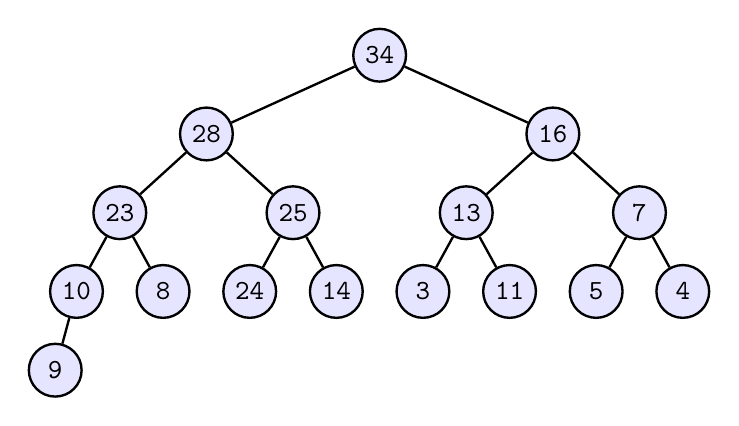
\begin{tikzpicture}

\fill[blue!10] (0.0, 0.0) circle (0.35);
\node [line width=0.03cm,black,minimum size=0.6699999999999999cm,draw,circle] at (0.0,0.0)(34){};\draw (0.0, 0.0) node[color=black] {\texttt{34}};
\fill[blue!10] (-2.2, -1.0) circle (0.35);
\node [line width=0.03cm,black,minimum size=0.6699999999999999cm,draw,circle] at (-2.2,-1.0)(28){};\draw (-2.2, -1.0) node[color=black] {\texttt{28}};
\fill[blue!10] (2.2, -1.0) circle (0.35);
\node [line width=0.03cm,black,minimum size=0.6699999999999999cm,draw,circle] at (2.2,-1.0)(16){};\draw (2.2, -1.0) node[color=black] {\texttt{16}};
\fill[blue!10] (-3.3, -2.0) circle (0.35);
\node [line width=0.03cm,black,minimum size=0.6699999999999999cm,draw,circle] at (-3.3,-2.0)(23){};\draw (-3.3, -2.0) node[color=black] {\texttt{23}};
\fill[blue!10] (-1.1, -2.0) circle (0.35);
\node [line width=0.03cm,black,minimum size=0.6699999999999999cm,draw,circle] at (-1.1,-2.0)(25){};\draw (-1.1, -2.0) node[color=black] {\texttt{25}};
\fill[blue!10] (1.1, -2.0) circle (0.35);
\node [line width=0.03cm,black,minimum size=0.6699999999999999cm,draw,circle] at (1.1,-2.0)(13){};\draw (1.1, -2.0) node[color=black] {\texttt{13}};
\fill[blue!10] (3.3, -2.0) circle (0.35);
\node [line width=0.03cm,black,minimum size=0.6699999999999999cm,draw,circle] at (3.3,-2.0)(7){};\draw (3.3, -2.0) node[color=black] {\texttt{7}};
\fill[blue!10] (-3.85, -3.0) circle (0.35);
\node [line width=0.03cm,black,minimum size=0.6699999999999999cm,draw,circle] at (-3.85,-3.0)(10){};\draw (-3.85, -3.0) node[color=black] {\texttt{10}};
\fill[blue!10] (-2.75, -3.0) circle (0.35);
\node [line width=0.03cm,black,minimum size=0.6699999999999999cm,draw,circle] at (-2.75,-3.0)(8){};\draw (-2.75, -3.0) node[color=black] {\texttt{8}};
\fill[blue!10] (-1.65, -3.0) circle (0.35);
\node [line width=0.03cm,black,minimum size=0.6699999999999999cm,draw,circle] at (-1.65,-3.0)(24){};\draw (-1.65, -3.0) node[color=black] {\texttt{24}};
\fill[blue!10] (-0.55, -3.0) circle (0.35);
\node [line width=0.03cm,black,minimum size=0.6699999999999999cm,draw,circle] at (-0.55,-3.0)(14){};\draw (-0.55, -3.0) node[color=black] {\texttt{14}};
\fill[blue!10] (0.55, -3.0) circle (0.35);
\node [line width=0.03cm,black,minimum size=0.6699999999999999cm,draw,circle] at (0.55,-3.0)(3){};\draw (0.55, -3.0) node[color=black] {\texttt{3}};
\fill[blue!10] (1.65, -3.0) circle (0.35);
\node [line width=0.03cm,black,minimum size=0.6699999999999999cm,draw,circle] at (1.65,-3.0)(11){};\draw (1.65, -3.0) node[color=black] {\texttt{11}};
\fill[blue!10] (2.75, -3.0) circle (0.35);
\node [line width=0.03cm,black,minimum size=0.6699999999999999cm,draw,circle] at (2.75,-3.0)(5){};\draw (2.75, -3.0) node[color=black] {\texttt{5}};
\fill[blue!10] (3.85, -3.0) circle (0.35);
\node [line width=0.03cm,black,minimum size=0.6699999999999999cm,draw,circle] at (3.85,-3.0)(4){};\draw (3.85, -3.0) node[color=black] {\texttt{4}};
\fill[blue!10] (-4.12, -4.0) circle (0.35);
\node [line width=0.03cm,black,minimum size=0.6699999999999999cm,draw,circle] at (-4.12,-4.0)(9){};\draw (-4.12, -4.0) node[color=black] {\texttt{9}};\draw[line width=0.03cm,black] (34) to  (28);
\draw[line width=0.03cm,black] (34) to  (16);
\draw[line width=0.03cm,black] (28) to  (23);
\draw[line width=0.03cm,black] (28) to  (25);
\draw[line width=0.03cm,black] (16) to  (13);
\draw[line width=0.03cm,black] (16) to  (7);
\draw[line width=0.03cm,black] (23) to  (10);
\draw[line width=0.03cm,black] (23) to  (8);
\draw[line width=0.03cm,black] (25) to  (24);
\draw[line width=0.03cm,black] (25) to  (14);
\draw[line width=0.03cm,black] (13) to  (3);
\draw[line width=0.03cm,black] (13) to  (11);
\draw[line width=0.03cm,black] (7) to  (5);
\draw[line width=0.03cm,black] (7) to  (4);
\draw[line width=0.03cm,black] (10) to  (9);
\end{tikzpicture}

\end{center}


from latextool_basic import *
print(automata(layout="""
A  B  E  F  

C  D  G  H
""",
edges="A,$a$,B|A,$b$,C|B,$a$,E|B,$b$,D|C,$b$,A|C,$a$,D|D,$b$,B|E,$a$,F|G,$a$,H|D,$a$,G|F,$a$,A|H,$a$,C|E,$b$,G|G,$b$,E|F,$b$,H|H,$b$,F",
A='initial|accept|label=$q_0$',
B='label=$q_1$',
C='accept|label=$q_4$',
D='label=$q_5$',
E='accept|label=$q_2$',
G='accept|label=$q_6$',
H='label=$q_7$',
F='label=$q_3$',
xscale=1.3,
))
\end{python}
\end{comment}
\begin{center}
\begin{tikzpicture}[>=triangle 60,shorten >=0.5pt,node distance=2cm,auto,initial text=]
\node[state,initial,accepting] (A) at (0.0,  0) {$q_0$};
\node[state] (B) at (3.9000000000000004,  0) {$q_1$};
\node[state,accepting] (E) at (7.800000000000001,  0) {$q_2$};
\node[state] (F) at (11.700000000000001,  0) {$q_3$};
\node[state] (C) at (0.0, -4) {$q_4$};
\node[state] (D) at (3.9000000000000004, -4) {$q_5$};
\node[state,accepting] (G) at (7.800000000000001, -4) {$q_6$};
\node[accepting,state] (H) at (11.700000000000001, -4) {$q_7$};

\path[->]
(A) edge [bend left=0,pos=0.5,above] node {$a$} (B)
(A) edge [bend left=10,pos=0.5] node {$b$} (C)
(B) edge [bend left=10,pos=0.5] node {$b$} (D)
(B) edge [bend left=0,pos=0.5,above] node {$a$} (E)
(C) edge [bend left=10,pos=0.5] node {$b$} (A)
(C) edge [bend left=0,pos=0.5,above] node {$a$} (D)
(D) edge [bend left=10,pos=0.5] node {$b$} (B)
(D) edge [bend left=0,pos=0.5,above] node {$a$} (G)
(E) edge [bend left=0,pos=0.5,above] node {$a$} (F)
(E) edge [bend left=10,pos=0.5] node {$b$} (G)
(F) edge [bend right=15,pos=0.5,above] node {$a$} (A)
(F) edge [bend left=10,pos=0.5] node {$b$} (H)
(G) edge [bend left=10,pos=0.5] node {$b$} (E)
(G) edge [bend left=0,pos=0.5,above] node {$a$} (H)
(H) edge [bend left=15,pos=0.5] node {$a$} (C)
(H) edge [bend left=10,pos=0.5] node {$b$} (F)

;
\end{tikzpicture}
\end{center}
Let $L = L(M)$.
\begin{enumerate}[label=\textnormal{(\alph*)},itemsep=0pt,nosep,noitemsep,partopsep=0pt,topsep=0pt,parsep=0pt]
\item Are $\ep,a^4$ $L$-distinguishable?
\item Are $\ep,a$ $L$-distinguishable?
\item Are $\ep,a^2$ $L$-distinguishable?
\item Are $\ep,a^3$ $L$-distinguishable?
\item Are $\ep,b$ $L$-distinguishable?
\item Are $\ep,ba$ $L$-distinguishable?
\item Are $\ep,ba^2$ $L$-distinguishable?
\item Are $\ep,ba^3$ $L$-distinguishable?
\end{enumerate}

\end{eg}


\newpage
Note that $L$--distinguishability does not depend on the concept of DFA.
The following is a pretty obvious statement on
the relationship between $L$--distinguishability and DFAs.
Let $\operatorname{state}_M(x)$ denotes the state that $x$ lands in
if $M$ computes with $x$, i.e.,
\[
\operatorname{state}_M(x) = \delta^*(q_0, x)
\]
where $q_0$ is the start state and
$\delta$ is the transition function 
of $M$.

\begin{prop}
  Let $M$ be a DFA and $L = L(M)$.
  Let $x, y \in \Sigma^*$ and $p,q$ be the respective states reached when
  $x,y$ are computed with $M$.
  If $x,y$ are $L$--distinguishable, then $\operatorname{state}_M(x) \neq \operatorname{state}_M(y)$. 
\end{prop}
\proof
The proof is obvious.
Suppose $x$ and $y$ lands in the same state.
Then for any $z \in \Sigma^*$, $xz$ and $yz$ will both also land in a common state.
Of course the state is either an accept state of non--accept state,
which means that $xz$ and $yz$ cannot be separated by $L$.
This contradicts the $L$--distinguishability of $x,y$.
\qed

\begin{prop}
  Let $L$ be a language.
  If $L = L(M)$ where $M$ is a DFA and $L$ has $k$ pairwise $L$--distinguishable strings,
  then $M$ has at least $k$ states.
\end{prop}
\proof
Let $x_0, \ldots, x_{k-1}$ be a set of $k$ pairwise $L$--distinguishable strings.
Suppose $M$ has less than $k$ states.
Running $M$ on the strings $x_0, \ldots, x_{k-1}$, we will obtain $k$ states.
By the pigeonhole principle, since $M$ has less than $k$ states,
two of the strings in $x_0, \ldots, x_{k-1}$ must land in the same state.
But this is a contradiction (by the previous statement) since $L$--distinguishable strings
cannot land in the same state.
\qed

\newpage
\begin{ex}
  \begin{tightlist}
  \item Let $L_1 = \{a^n b^n \mid n \geq 0\}$.
    Prove that $L_1$ is not a regular language.
  \item
    Let $L_2 = \{w \in \Sigma^* \mid |w|_a, |w|_b \text{ both even}\}$.
    What is the size of the smallest DFA?
    Construct a minimal DFA for $L_2$.
    Note that the results above only tells you a lower bound
    on the number of states of a DFA for $L_2$.
    It does not say that the number stated is attained.
    The results above also does not tell you how to construct a DFA.
  \end{tightlist}
\end{ex}

\newpage
Note that the previous statements tell you when you have the smallest DFA for a language.
But suppose a language has $5$ distinguishable strings.
At this point, you only know that a DFA has at least 5 states.
Does the minimal DFA have \textit{exactly} 5?
The above statement does not address this question.

Another thing to note is that we already have many techniques for
designing DFAs.
What we need is to use those techniques to build a DFA, and \textit{then} minimize \textit{that} DFA just built.

So here we go ...

First, recall that I have a relation $\equiv_L$ on strings in $\Sigma^*$.
Recall that $\not\equiv_L$ means $L$--distinguishability.
In other words
\[
x \not\equiv_L y
\]
if there is some $z \in\Sigma^*$ such that $L$ separates $xz,yz$.
In other words
\[
x \equiv_L y
\]
if for all $z \in\Sigma^*$, $L$ does not separate $xz,yz$.

\begin{prop}
  $\equiv_L$ is an equivalence relation on $\Sigma^*$.
  In other words:
  \begin{tightlist}
    \item[\textnormal{(a)}] Reflexivity: For all $x \in \Sigma^*$, $x \equiv_L x$. 
    \item[\textnormal{(b)}] Symmetry: For all $x,y \in \Sigma^*$, if $x \equiv_L y$, then $y \equiv_L x$. 
    \item[\textnormal{(c)}] Transitivity: For all $x,y,w \in \Sigma^*$, if $x \equiv_L y, y \equiv_L w$, then $x \equiv_L w$. 
  \end{tightlist}
\end{prop}
\proof
Easy exercise.
\qed

This means that $\Sigma^*$ is partitioned into a collection of disjoint sets of strings.
The fancy term for such a set is \defone{equivalence class}.
In other words the collection of equivalence classes look like
$
[x_0],
[x_1],
[x_2],...,
[x_{k-1}]
$
where
\[
[x_i] = \{x \in \Sigma^* \mid x_i \equiv_L x \}
\]
Here's I'm assuming the number of equivalence classes is finite.
It can be infinite -- see exercise on showing $L_1 = \{a^n b^n \mid n \geq 0\}$ is not regular.

Remember what I said: If there are $k$ equivalence classes,
it means that a DFA for $L$ (if there's one at all) has at least $k$ states.
It turns out the $k$ \textit{is} actually the correct number of states for the smallest DFA:

\begin{thm} \defone{\textnormal{Myhill--Nerode (1958)}}
  Let $L$ be a language (over $\Sigma^*)$.
  \begin{tightlist}
  \item[\textnormal{(a)}] If $\equiv_L$ (over $\Sigma^*$) has infinitely many equivalence classes
    then $L$ is not regular.
  \item[\textnormal{(b)}] If $\equiv_L$ (over $\Sigma^*$) has finitely many equivalence classes, say $k$,
    then $L$ is regular and there is a DFA $M$ with exactly $k$ states, where each state
    correspond to an equivalence class of $\equiv_L$.
    Specifically if
    $
    [x_0],
    [x_1],
    [x_2],...,
    [x_{k-1}]
    $
    where $x_0 = \ep$,
    are the equivalence classes of $\equiv_L$, then we 
    define $M = (\Sigma, Q, q_0, F, \delta)$ to be
    \begin{tightlist}
    \item The set of states $Q$ is $\{[x_0], [x_1], [x_2],..., [x_{k-1}]\}$.
    \item The start state is $[x_0]$.
    \item The set of final states $F$ consists of those $[x_i]$ where $x_i \in L$.
    \item The transition function $\delta : Q \times \Sigma \rightarrow Q$ is defined as follows.
      If $c \in \Sigma$,
      \[
      \delta([x_i], c) = [x_i c]
      \]
    \end{tightlist}
    then $L(M) = L$.
  \end{tightlist}
\end{thm}


Before proving Myhill--Nerode's theorem, let me use it ...

\newpage
\begin{eg}
  Let's try to compute the minimal DFA for
  \[
  L_2 = \{w \in \Sigma^* \mid |w|_a, |w|_b \text{ both even}\}
  \]
\end{eg}

\SOLUTION
Recall from the earlier exercises, there are exactly four $L_2$--distinguishable strings:
\[
\ep, a, b, ab
\]
Hence $\equiv_{L_2}$ partitions $\Sigma^*$ into four equivalence classses:
\[
  [\ep], [a], [b], [ab]
\]
where
\begin{align*}
  [\ep] &= \{x \in \Sigma^* \mid \ep \equiv_L x \} = \{x \in \Sigma^* \mid |x|_a,|x|_b \equiv 0,0 \pmod{2} \} \\
  [a] &= \{x \in \Sigma^* \mid a \equiv_L x \} = \{x \in \Sigma^* \mid |x|_a,|x|_b \equiv 1,0 \pmod{2} \} \\
  [b] &= \{x \in \Sigma^* \mid b \equiv_L x \} = \{x \in \Sigma^* \mid |x|_a,|x|_b \equiv 0,1 \pmod{2} \} \\
  [ab] &= \{x \in \Sigma^* \mid ab \equiv_L x \} = \{x \in \Sigma^* \mid |x|_a,|x|_b \equiv 1,1 \pmod{2} \}
\end{align*}
The start state is $[\ep]$.
The set of accept states is
\[
F = \{[\ep]\}
\]
since among the string $\ep, a, b, ab$, $\ep$ is the
only string in $L$.
The transition function $\delta$ is given by the following:
\begin{enumerate}[label=\textnormal{(\alph*)},itemsep=0pt,nosep,noitemsep,partopsep=0pt,topsep=0pt,parsep=0pt]
  \li $\delta([\ep], a) = [\ep a] = [a]$.
  \li $\delta([\ep], b) = [\ep b] = [b]$.
  \li $\delta([a], a) = [aa] = [\ep]$. This is because $aa \equiv_{L_2} \ep$.
  \li $\delta([a], b) = [ab]$.
  \li $\delta([b], a) = [ba] = [ab]$. This is because $ba \equiv_{L_2} ab$.
  \li $\delta([b], b) = [bb] = [\ep]$. This is because $bb \equiv_{L_2} \ep$.
  \li $\delta([ab], a) = [aba] = [b]$. This is because $aba \equiv_{L_2} b$.
  \li $\delta([ab], b) = [abb] = [a]$. This is because $abb \equiv_{L_2} a$.
\end{enumerate}
The above describes the DFA completely.
Here's the diagram:

\begin{center}
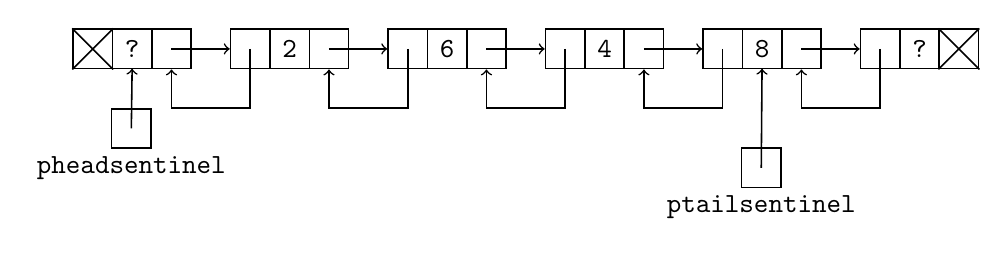
\begin{tikzpicture}

\draw (0.25, 0.25)
  node[draw, line width=0.02cm, , color=black,
       rounded corners=0cm, inner sep=0cm] {

\begin{minipage}[t][0.5cm]{0.5cm}
\mbox{}

\end{minipage}

};\draw (0.25, 0.25) node[color=black] {{\texttt{}}};
\draw (0.75, 0.25)
  node[draw, line width=0.02cm, , color=black,
       rounded corners=0cm, inner sep=0cm] {

\begin{minipage}[t][0.5cm]{0.5cm}
\mbox{}

\end{minipage}

};\draw (0.75, 0.25) node[color=black] {{\texttt{?}}};
\draw (1.25, 0.25)
  node[draw, line width=0.02cm, , color=black,
       rounded corners=0cm, inner sep=0cm] {

\begin{minipage}[t][0.5cm]{0.5cm}
\mbox{}

\end{minipage}

};\draw (1.25, 0.25) node[color=black] {{\texttt{}}};
\draw (2.25, 0.25)
  node[draw, line width=0.02cm, , color=black,
       rounded corners=0cm, inner sep=0cm] {

\begin{minipage}[t][0.5cm]{0.5cm}
\mbox{}

\end{minipage}

};\draw (2.25, 0.25) node[color=black] {{\texttt{}}};
\draw (2.75, 0.25)
  node[draw, line width=0.02cm, , color=black,
       rounded corners=0cm, inner sep=0cm] {

\begin{minipage}[t][0.5cm]{0.5cm}
\mbox{}

\end{minipage}

};\draw (2.75, 0.25) node[color=black] {{\texttt{2}}};
\draw (3.25, 0.25)
  node[draw, line width=0.02cm, , color=black,
       rounded corners=0cm, inner sep=0cm] {

\begin{minipage}[t][0.5cm]{0.5cm}
\mbox{}

\end{minipage}

};\draw (3.25, 0.25) node[color=black] {{\texttt{}}};
\draw (4.25, 0.25)
  node[draw, line width=0.02cm, , color=black,
       rounded corners=0cm, inner sep=0cm] {

\begin{minipage}[t][0.5cm]{0.5cm}
\mbox{}

\end{minipage}

};\draw (4.25, 0.25) node[color=black] {{\texttt{}}};
\draw (4.75, 0.25)
  node[draw, line width=0.02cm, , color=black,
       rounded corners=0cm, inner sep=0cm] {

\begin{minipage}[t][0.5cm]{0.5cm}
\mbox{}

\end{minipage}

};\draw (4.75, 0.25) node[color=black] {{\texttt{6}}};
\draw (5.25, 0.25)
  node[draw, line width=0.02cm, , color=black,
       rounded corners=0cm, inner sep=0cm] {

\begin{minipage}[t][0.5cm]{0.5cm}
\mbox{}

\end{minipage}

};\draw (5.25, 0.25) node[color=black] {{\texttt{}}};
\draw (6.25, 0.25)
  node[draw, line width=0.02cm, , color=black,
       rounded corners=0cm, inner sep=0cm] {

\begin{minipage}[t][0.5cm]{0.5cm}
\mbox{}

\end{minipage}

};\draw (6.25, 0.25) node[color=black] {{\texttt{}}};
\draw (6.75, 0.25)
  node[draw, line width=0.02cm, , color=black,
       rounded corners=0cm, inner sep=0cm] {

\begin{minipage}[t][0.5cm]{0.5cm}
\mbox{}

\end{minipage}

};\draw (6.75, 0.25) node[color=black] {{\texttt{4}}};
\draw (7.25, 0.25)
  node[draw, line width=0.02cm, , color=black,
       rounded corners=0cm, inner sep=0cm] {

\begin{minipage}[t][0.5cm]{0.5cm}
\mbox{}

\end{minipage}

};\draw (7.25, 0.25) node[color=black] {{\texttt{}}};
\draw (8.25, 0.25)
  node[draw, line width=0.02cm, , color=black,
       rounded corners=0cm, inner sep=0cm] {

\begin{minipage}[t][0.5cm]{0.5cm}
\mbox{}

\end{minipage}

};\draw (8.25, 0.25) node[color=black] {{\texttt{}}};
\draw (8.75, 0.25)
  node[draw, line width=0.02cm, , color=black,
       rounded corners=0cm, inner sep=0cm] {

\begin{minipage}[t][0.5cm]{0.5cm}
\mbox{}

\end{minipage}

};\draw (8.75, 0.25) node[color=black] {{\texttt{8}}};
\draw (9.25, 0.25)
  node[draw, line width=0.02cm, , color=black,
       rounded corners=0cm, inner sep=0cm] {

\begin{minipage}[t][0.5cm]{0.5cm}
\mbox{}

\end{minipage}

};\draw (9.25, 0.25) node[color=black] {{\texttt{}}};
\draw (10.25, 0.25)
  node[draw, line width=0.02cm, , color=black,
       rounded corners=0cm, inner sep=0cm] {

\begin{minipage}[t][0.5cm]{0.5cm}
\mbox{}

\end{minipage}

};\draw (10.25, 0.25) node[color=black] {{\texttt{}}};
\draw (10.75, 0.25)
  node[draw, line width=0.02cm, , color=black,
       rounded corners=0cm, inner sep=0cm] {

\begin{minipage}[t][0.5cm]{0.5cm}
\mbox{}

\end{minipage}

};\draw (10.75, 0.25) node[color=black] {{\texttt{?}}};
\draw (11.25, 0.25)
  node[draw, line width=0.02cm, , color=black,
       rounded corners=0cm, inner sep=0cm] {

\begin{minipage}[t][0.5cm]{0.5cm}
\mbox{}

\end{minipage}

};\draw (11.25, 0.25) node[color=black] {{\texttt{}}};\draw[line width=0.02cm,black,->] (1.25,0.25) to  (1.99,0.25);
\draw[line width=0.02cm,black,->] (3.25,0.25) to  (3.99,0.25);
\draw[line width=0.02cm,black,->] (2.25,0.25) to  (2.25,-0.5) to  (1.25,-0.5) to  (1.25,-0.01);
\draw[line width=0.02cm,black,->] (5.25,0.25) to  (5.99,0.25);
\draw[line width=0.02cm,black,->] (4.25,0.25) to  (4.25,-0.5) to  (3.25,-0.5) to  (3.25,-0.01);
\draw[line width=0.02cm,black,->] (7.25,0.25) to  (7.99,0.25);
\draw[line width=0.02cm,black,->] (6.25,0.25) to  (6.25,-0.5) to  (5.25,-0.5) to  (5.25,-0.01);
\draw[line width=0.02cm,black,->] (9.25,0.25) to  (9.99,0.25);
\draw[line width=0.02cm,black,->] (8.25,0.25) to  (8.25,-0.5) to  (7.25,-0.5) to  (7.25,-0.01);
\draw[line width=0.02cm,black,->] (10.25,0.25) to  (10.25,-0.5) to  (9.25,-0.5) to  (9.25,-0.01);
\draw[line width=0.02cm,black] (-0.01,0.51) to  (0.51,-0.01);
\draw[line width=0.02cm,black] (0.51,0.51) to  (-0.01,-0.01);
\draw[line width=0.02cm,black] (10.99,0.51) to  (11.51,-0.01);
\draw[line width=0.02cm,black] (11.51,0.51) to  (10.99,-0.01);

\draw (0.74, -0.76)
  node[draw, line width=0.02cm, , color=black,
       rounded corners=0cm, inner sep=0cm] {

\begin{minipage}[t][0.5cm]{0.5cm}
\mbox{}

\end{minipage}

};\draw (0.74, -0.76) node[color=black] {{\texttt{}}};
\draw (0.74, -1.26)
  node[draw, line width=0.02cm, , color=white,
       rounded corners=0cm, inner sep=0cm] {

\begin{minipage}[t][0.1cm]{0.1cm}
\mbox{}

\end{minipage}

};\draw (0.74, -1.26) node[color=black] {{\texttt{pheadsentinel}}};\draw[line width=0.02cm,black,->] (0.74,-0.76) to  (0.75,0);

\draw (8.74, -1.26)
  node[draw, line width=0.02cm, , color=black,
       rounded corners=0cm, inner sep=0cm] {

\begin{minipage}[t][0.5cm]{0.5cm}
\mbox{}

\end{minipage}

};\draw (8.74, -1.26) node[color=black] {{\texttt{}}};
\draw (8.74, -1.76)
  node[draw, line width=0.02cm, , color=white,
       rounded corners=0cm, inner sep=0cm] {

\begin{minipage}[t][0.1cm]{0.1cm}
\mbox{}

\end{minipage}

};\draw (8.74, -1.76) node[color=black] {{\texttt{ptailsentinel}}};\draw[line width=0.02cm,black,->] (8.74,-1.26) to  (8.75,0);
\end{tikzpicture}

\end{center}


from latextool_basic import *
print(automata(layout="""
A  B

C  D
""",
edges="A,$a$,B|A,$b$,C|B,$b$,D|B,$a$,A|C,$a$,D|C,$b$,A|D,$a$,C|D,$b$,B",
A='initial|label=$[\ep]$',
B='label=$[a]$',
C='label=$[b]$',
D='accept|label=$[ab]$',
xscale=1.2
))
\end{python}

\newpage

Now let's prove Myhill--Nerode's theorem.

\proof
(a) If $\equiv_L$ has infinitely many equivalence classes, that means that there are
infinitely many $L$--distinguishable strings and we have already mentioned that
this means that for every $k > 0$, a DFA for $L$ (if it exists) must have at least $k$ states.
But this means that $M$ has arbitrarily many states.
That's impossible since $M$ must have a finite number of states by definition.
(I actually already talked about this earlier.)

(b)
First let me show that $\delta$ is well--defined, i.e.,
I need to show that if $x_i \equiv_L x$, then
\[
\delta([x_i], c) = [x_i c] = [x'c] = \delta([x], c)
\]
In other words, I need to show
\[
  x_i c \equiv_L x'c
\]
Again, I need to show
\[
x_i \equiv_L x \implies x_i c \equiv_L x'c 
\]
$x_i \equiv_L x$ means that for all $z \in \Sigma^*$,
$L$ does not separate $x_iz, xz$.
Let $z' \in \Sigma^*$.
Then $x_i(cz'), x(cz)$ are not separated by $L$.
Hence $(x_ic)z', (xc)z$ are not separated by $L$,
which implies that $x_ic, xc$ are not $L$--distinguishable, i.e.,
$x_ic \equiv_L xc$.

Clearly $M$ is a DFA.
Now I need to show $L(M) = L$.
Let $x \in \Sigma^*$.
\begin{align*}
  x \in L(M) \iff \delta^*([\ep], x) \in F
\end{align*}
Note that
\[
\delta^*([\ep], x) = [x]
\]
for any $x \in \Sigma^*$. (This can be proven by induction.)
Hence
\begin{align*}
  x \in L(M)
  &\iff [x] \in F \\
  &\iff \exists x_i \in L \text{ such that } [x] = [x_i] \\
  &\iff \exists x_i \in L \text{ such that } x \equiv_L x_i \\
  &\iff \exists x_i \in L \text{ such that } \forall z,
  L \text{ does not separate }
  xz, x_iz 
\end{align*}
In particular, if $x \in L(M)$, then
there is some $x_i \in L$ such that for $z = \ep$,
$xz=x$ and $x_iz=x_i$ are not $L$ separable.
Since $x_i \in L$ and $L$ does not separate $x,x_i$, $x \in L$.
I have just shown
\[
x \in L(M) \implies x \in L
\]
Hence $L(M) \subseteq L$.
Now let $x \in L$, say $[x] = [x_i]$.
\[
\delta^*([\ep], x) = [x] = [x_i] 
\]
This implies that for all $z$, $L$ does not separate
$xz,x_iz$.
In particular when $z = \ep$,
$L$ does not separate
$x,x_i$.
Since $x \in L$, then $x_i \in L$.
Hence
\[
\delta^*([\ep], x) = [x] = [x_i] \in F
\]
Therefore $x \in L$. Hence $L \subseteq L(M)$.
Altogether I have shown $L = L(M)$.
\qed


The easiest thing to do is to remove states which are not
reachable from the start state.
Simply perform a breadth-first traversal.
For instance (this is not optimized):
\begin{console}
Let S be the set of reachable states. Initialize is with the start state.

Repeatedly, put all states reachable from S into S.
Repeat the above until S is not changed.
\end{console}
After the above is done, only the states in $S$ need to be
considered.
The states in $Q - S$ are thrown away.
Of course $F$ is replaced by $F - S$ and $\delta$ is
updated so that only states in $Q - S$ are considered part of $\delta$.

First we'll find a smaller DFA. Later we'll prove that it's the
smallest using Myhill-Nerode's Theorem.

Throughout this section, $M = (\Sigma,Q,q_0,F,\delta)$ will be a $\DFA$
where $Q = \{q_0,\ldots,q_{n-1}\}$

The idea is to collapse states $\ldots$ equivalence relations to
the rescue!


Let $L$ be a language (over $\Sigma$).
Given two strings $x,y$ in $\Sigma^*$, I will say
that $L$ separates $x,y$ if
there is some $z \in \Sigma^*$ such that 
either
$xz \in L, yz \not\in L$
or 
$xz \not\in L, yz \in L$.
I will further write
\[
x \equiv_L y
\]
if there is no $z$ such that $L$ separates $xz,yz$.
In other words
\[
x \equiv_L y
\]
iff
\[
\text{for all } z \in \Sigma^*, xz \in L \iff yz \in L
\]


\begin{prop}
$\equiv_L$ is an equivalence relation on $\Sigma^*$
\end{prop}
\proof
Exercise.
\qed


What is the intuition here?


Consider the example of
\[
L = \{ x \in \{a,b\}^* \mid |x| \equiv 1 \bmod{8}\}
\]
Let $M$ be the DFA with 8 states that accepts
$w \in \Sigma^* = \{a, b\}^*$ where the number of
$a$'s in $w$ is $\equiv 1$ or $5 \pmod{8}$.
We do know that $L$ is regular with a DFA with 8 states.
Notice that the string $\Sigma^*$ will land in the states.
So we can think of classes of strings as being same as states, i.e.,
each state can be thought of as a collection of strings from $\Sigma^*$.
For instance if $|x| = 6$ and $|y| = 8k + 6$, then
\[
x \equiv_L
\]
Hence $\Sigma^*$ is partitioned into 8 sets of strings in the obvious way.
The partitions are
\begin{tightlist}
  \li $[\ep]$
  \li $[a] = [b]$
  \li $[a^2] = [b^2] = [ab] = [ba]$
  \li $[a^3] = [b^3]$
  \li $[a^4]$
  \li $[a^5]$
  \li $[a^6]$
  \li $[a^7]$
\end{tightlist}

\newpage
\begin{ex}
Prove that $\equiv_M$ is an equivalence relation on $\Sigma^*$.
Therefore $\Sigma^*$ is partitioned into equivalence classes of
strings. We will write $[x]_M$ for the equivalence class containing
$x$, i.e.,
\[
 [x]_M = \{ y \in \Sigma^* \,|\, x \equiv_M y \}
\]
We will write $\ind(\equiv_M)$ for the number of equivalence classes
of $\Sigma^*$ under $\equiv_M$.
\end{ex}

$\equiv_M$ is more than just an equivalence relation. Note that if
$x \equiv_M y$, then they remain equivalence (wrt $\equiv$) even
when you extend them ``on their right":


\begin{ex}
Let $M$ be a $\DFA$. Prove that $\equiv_M$ is right invariant.
\qed
\end{ex}

The main idea is that the equivalence classes of $L$ under
$\equiv_M$ will be the states. [?]

Now we define an equivalence relation on \textit{any} language $L$.
Note that $L$ need not be regular:

\begin{defn}
  Let $L$ be any language.
  Define the following relation on $\Sigma^*$.
  For $x,y \in \Sigma^*$, 
  \[
  x \equiv_L y \,\,\, \text{ if } \,\,\,\text{for all $z$, } xz \in L
  \iff yz \in L
  \]  
  This is the same as saying that $x \equiv_L y$ if for all $z \in
  \Sigma^*$, either
  \begin{itemize}
  \item $xz, yz$ both in $L$, or
  \item $xz, yz$ both not in $L$.
  \end{itemize}
  
  We will write $[x]_L$ for the equivalence class of $x$ under
  $\equiv_L$.

\end{defn}



\begin{eg}
Let $\Sigma = \{a,b\}$. For simplicity we will write $|w|_a$ for the
number of $a$'s in $w$ and $|w|_b$ for the number of $b$'s in $w$.
Let $L = \{w \in \Sigma^* \,|\, |w|_a, |w|_b \text{ are even} \}$.

Look at the conditions: $|w|_a$ is even and $|w|_b$ is even. Notice
that if you define the following sets
 \begin{tightlist}
  \item $L_{ee} = \{w \in \Sigma^* \,|\, |w|_a \text{ even}, |w|_b \text{
  even}\}$
 \item $L_{eo} = \{w \in \Sigma^* \,|\, |w|_a \text{ even}, |w|_b \text{
  odd}\}$
  \item $L_{oe} = \{w \in \Sigma^* \,|\, |w|_a \text{ odd}, |w|_b \text{
  even}\}$
 \item $L_{oo} = \{w \in \Sigma^* \,|\, |w|_a \text{ even}, |w|_b \text{
  even}\}$
 \end{tightlist}

Obviously $L_{ee}, L_{eo}, L_{oe}, L_{oo}$ forms a partition of $L$
(Recall: this means they are pairwise disjoint and their union is
$L$.)

When we look the equivalence relation on $L$, we see that
 \begin{tightlist}
  \item $L_{ee} = [\ep]$
  \item $L_{eo} = [b]$
  \item $L_{oe} = [aaabb]$
  \item $L_{oo} = [baaabb]$
 \end{tightlist}

Not only that, we can actually use these equivalence classes of
strings to create a $\DFA$ in the following way. If $x \in \Sigma^*$
and $a \in \Sigma$, we just define
\[
  \delta([x]_L, a) = [xa]_L
\]

This is the smallest (in terms of number of states) DFA that accepts
$L$.
\end{eg}

\begin{eg}
Now consider $L = \{w \in \Sigma \,|\, w \text{ does not contain aab
}\}$ where $\Sigma = \{a,b\}$.
 \begin{itemize}
  \item Is $ba \equiv_L baa$?
  \item Suppose $w,w'$ both contain $aab$. Is it true that $w \equiv
 _L w'$?
 \end{itemize}
\end{eg}

OK. Here's the big theorem of this section:

\begin{thm} (Myhill-Nerode) \label{T:myhillnerode} Let $L$ be a language over
$\Sigma$.
The following are equivalent:
 \begin{itemize}
  \item[(a)] $L$ is regular
  \item[(b)] There is a right invariant equivalence relation $\equiv$  on $L$
   such that $\equiv$ has finite index and $L$ is the union of some
   equivalence classes of $\equiv$.
  \item[(c)] $\equiv_L$ has finite index.
 \end{itemize}
\end{thm}

I will not give a proof. However the important thing is that the
proof of (c) $\implies$ (a) is constructive. In particular, the DFA
constructed uses equivalence classes of $\equiv_L$ as states.

The important thing you should realize by reading this theorem is
that this is another way of characterizing regular languages. This
characterization does not rely on the definition of DFA. In other
words you can now re-define what is meant by regular in terms of
$\equiv_L$ and the finiteness of the equivalence classes of
$\equiv_L$. Theorems like these are extremely important because they
reveal connections between different concepts and reveal different
points of view. Note also that if you can write down infinitely many
strings which are not equivalent to each other, then $L$ is not
regular.

\begin{thm} (DFA Minimization) \label{T:dfaminimization}
 If $L$ is regular and $M$ is a DFA with the minimum number of
 states, then $M$ is the ``same" as the DFA constructed in the
 Myhill-Nerode theorem.
\end{thm}

Here ``same" can be formalize in terms of isomorphisms of DFA. It
means ``the same up to renaming the states". For instance if you
take a DFA with states labeled $q_0, q_1, \ldots, q_{n-1}$ and
relabel them as $s_0, s_1, \ldots, s_{n-1}$, then obviously the way
they both operate is exactly the same except for the names of the
states.

The important thing for us is how do we simplify a DFA? First of all
the simplest thing to do first is to remove states that cannot be
reached from the initial state. For a human being, if the DFA is
simple, then we can do it visually. In terms of an algorithm, you
need to process the states in the following manner. First you need a
list of states called $B$. This will be the list of states you will
visit. You also need a list of visited states; let's call this $A$.
You initialize $B$ with the initial state and initialize $A$ to be
empty. Now in a while loop, take a state $q$ out of $B$, visit all
the states you can go to from $q$ and put them into $B$, and put $q$
into $A$. Repeat this loop as long as $B$ is not empty. When you're
done, $A$ contains all the states that can be reached from the
initial state.

The other question is how do we merge the visited states?

We will define another relation on states $\equiv$ so that states
that should merge are equivalence to each other. Let $p,q$ be
states. Then we say that $p$ and $q$ are indistinguishable, and we
write
\[
 p \equiv q
\]
if there is some $z$ such that either
\begin{itemize}
 \item $\delta(p,z) \in F$ and $\delta(q,z) \notin F$, or
 \item $\delta(p,z) \notin F$ and $\delta(q,z) \in F$
 \end{itemize}
All you need to do is to merge indistinguishable states into a new
state.

Here's a systematic way of telling if pairs of states are
distinguishable or not:

[insert]

There is a more efficient algorithm (I won't do it here) that will
build the minimum DFA with time complexity $O(n \lg n)$ where $n =
|Q|$.
